\documentclass[aspectratio=169,12pt,t]{beamer}

% --- Theme: Metropolis (modern, clean) ---
\usetheme[progressbar=frametitle,numbering=fraction,block=fill]{metropolis}

% --- Fira Sans font (install texlive-fonts-extra if missing) ---
\IfFileExists{FiraSans.sty}{\usepackage[sfdefault]{FiraSans}}{}

% --- Light background with warm accent ---
\definecolor{mDarkTeal}{RGB}{35,55,59}
\definecolor{mLightBrown}{RGB}{235,228,216}
\definecolor{mAccent}{RGB}{140,70,20}

\setbeamercolor{normal text}{fg=mDarkTeal,bg=white}
\setbeamercolor{alerted text}{fg=mAccent}
\setbeamercolor{frametitle}{bg=mDarkTeal,fg=white}
\setbeamercolor{progress bar}{fg=mAccent,bg=mLightBrown}
\setbeamercolor{title separator}{fg=mAccent}
\setbeamercolor{progress bar in head/foot}{fg=mAccent,bg=mLightBrown}
\setbeamercolor{progress bar in section page}{fg=mAccent,bg=mLightBrown}

% --- Packages ---
\usepackage[utf8]{inputenc}
\usepackage{amsmath,amssymb,amsthm}
\usepackage{mathrsfs}
\usepackage{tikz}
\usetikzlibrary{arrows.meta,positioning,calc,decorations.pathreplacing,shapes,patterns}
\usepackage{pgfplots}
\pgfplotsset{compat=1.18}

% --- TikZ diagram styles (shared across the series) ---
\tikzset{
  axisln/.style={-{Stealth[length=2.6mm]}, line width=0.8pt, gray!75},
  curveln/.style={line width=1.6pt, line cap=round, line join=round},
  projln/.style={dash pattern=on 2.6pt off 2pt, line width=0.7pt},
  guide/.style={-{Stealth[length=2.6mm,width=2.2mm]}, line width=1.1pt},
}
% point marker with a white halo: \dotpt{color}{(coord)}
\newcommand{\dotpt}[2]{%
  \fill[white] #2 circle (3.6pt);
  \fill[#1] #2 circle (2.4pt);
}
% open point marker: \opendotpt{color}{(coord)}
\newcommand{\opendotpt}[2]{%
  \fill[white] #2 circle (3.6pt);
  \draw[#1, line width=1pt] #2 circle (2.4pt);
}

% --- Semi-transparent white highlight for text on top of background images ---
\usepackage[most]{tcolorbox}

% Inline highlight: \hl{short text}
\newtcbox{\hl}{%
  nobeforeafter, tcbox raise base,
  colback=white, opacityback=0.6,
  colframe=white, opacityframe=0,
  sharp corners, boxsep=2pt, left=3pt, right=3pt, top=2pt, bottom=2pt%
}

% Block highlight: \begin{hlbox} ... \end{hlbox}  (multi-line, paragraphs, itemize)
% Optional argument accepts any tcolorbox key, e.g. [width=0.6\linewidth]
\newtcolorbox{hlbox}[1][]{%
  enhanced, breakable,
  colback=white, opacityback=0.6,
  colframe=white, opacityframe=0,
  boxsep=3pt, left=6pt, right=6pt, top=4pt, bottom=4pt,
  sharp corners,
  {#1}%
}

% --- Custom colors for content types ---
\definecolor{defcolor}{RGB}{25,85,120}
\definecolor{thmcolor}{RGB}{140,35,35}
\definecolor{proofcolor}{RGB}{35,100,50}
\definecolor{excolor}{RGB}{140,75,10}
\definecolor{remcolor}{RGB}{90,90,90}

% --- Beamer blocks for mathematical content types (semi-transparent) ---
\tcbset{hlblockbase/.style={
  enhanced, breakable,
  coltitle=white, fonttitle=\bfseries,
  opacitybacktitle=0.8, opacityback=0.6,
  opacityframe=0,
  sharp corners,
  boxsep=1pt, left=5pt, right=5pt, top=2pt, bottom=2pt,
  toptitle=1pt, bottomtitle=1pt
}}

\newtcolorbox{defblock}[1]{hlblockbase, title={#1},
  colbacktitle=defcolor, colback=defcolor!15, colframe=defcolor}
\newtcolorbox{thmblock}[1]{hlblockbase, title={#1},
  colbacktitle=thmcolor, colback=thmcolor!15, colframe=thmcolor}
\newtcolorbox{proofblock}[1]{hlblockbase, title={#1},
  colbacktitle=proofcolor, colback=proofcolor!15, colframe=proofcolor}
\newtcolorbox{exblock}[1]{hlblockbase, title={#1},
  colbacktitle=excolor, colback=excolor!15, colframe=excolor}
\newtcolorbox{remblock}[1]{hlblockbase, title={#1},
  colbacktitle=remcolor, colback=remcolor!15, colframe=remcolor}

% --- Metadata ---
\title{Chapter 5: Differentiation}
\subtitle{Section: Differentiation of Vector-Valued Functions}
\author{Based on Walter Rudin's \emph{Principles of Mathematical Analysis}}
\date{}

\begin{document}

{
\usebackgroundtemplate{%
  
\includegraphics[width=\paperwidth,height=\paperheight,keepaspectratio=false]{chapter_05_bg_00.png}%
}
\begin{frame}[plain]
  \titlepage

  \note{
    Welcome to Chapter 5, Section 7: Differentiation of Vector-Valued
    Functions. This is the final episode of the chapter, and it has the
    flavor of a plot twist. So far, every function in Chapter 5 has been
    real-valued: the derivative, the mean value theorems, Lopital's rule,
    and Taylor's theorem were all stated for functions taking values on
    the real line. Today we ask what happens when the values are complex
    numbers, or more generally points of a higher dimensional space.
    Some of our results survive without changing a single word. But two
    of the most famous ones, the mean value theorem and Lopital's rule,
    fail, and we will see two beautiful counterexamples.
    The episode ends on a happy note: Theorem 5.19, an inequality that
    salvages everything we actually need from the mean value theorem.
    Let's get started.
  }
\end{frame}
}

{
\usebackgroundtemplate{%
  
\includegraphics[width=\paperwidth,height=\paperheight,keepaspectratio=false]{chapter_05_bg_01.png}%
}
\begin{frame}[c]{Outline}
  \begin{center}
    \tableofcontents
  \end{center}

  \note{
    Here is the plan for this episode. We begin with motivation: why we
    want to differentiate functions whose values are vectors, and what
    is at stake. We then extend the derivative itself, first to complex
    valued functions and then to functions with values in "k"
    dimensional space; this is the content of Remarks 5.16, and the
    extension turns out to be completely painless. The drama comes next.
    Example 5.17 shows that the mean value theorem fails for complex
    valued functions, and Example 5.18 shows that Lopital's rule fails
    as well. In the last part we prove Theorem 5.19, the mean value
    inequality, which survives in the vector setting and is, for
    applications, almost as good as the original theorem. We close with
    a summary and a look ahead at Chapter 6.
  }
\end{frame}

\section{Motivation}

% --- Build 1/3 ---
\begin{frame}{Beyond Real-Valued Functions}
  \begin{hlbox}
  \begin{itemize}
    \item So far in Chapter 5: $f\colon [a,b] \to \mathbb{R}$ ---
      derivative, mean value theorems, L'Hospital's rule, Taylor's theorem
  \end{itemize}
  \end{hlbox}

  \note{
    Let's take stock of where we are. Everything we have proved in this
    chapter, the definition of the derivative, the mean value theorems,
    Lopital's rule, and Taylor's theorem, was stated for functions
    defined on an interval and taking values on the real line. The
    real-valued assumption was quietly built into every proof. It is
    natural to ask how much of this machinery depends on it.
  }
\end{frame}

% --- Build 2/3 ---
\begin{frame}{Beyond Real-Valued Functions}
  \begin{hlbox}
  \begin{itemize}
    \item So far in Chapter 5: $f\colon [a,b] \to \mathbb{R}$ ---
      derivative, mean value theorems, L'Hospital's rule, Taylor's theorem
    \item Many natural functions are \alert{vector-valued}:
      complex $f = f_1 + i f_2$, \ curves
      $\mathbf{f}\colon [a,b] \to \mathbb{R}^k$
  \end{itemize}
  \end{hlbox}

  \note{
    And the question matters, because many natural functions are not
    real-valued at all. A complex valued function "f" is a pair of real
    functions, its real part "f" sub 1 and its imaginary part "f" sub 2,
    glued together. More generally, a function from an interval into
    "R" to the power "k" describes a curve, like the position of a
    moving particle: at each time "t" the value is a point in space,
    not a number. We would like to differentiate these too.
  }
\end{frame}

% --- Build 3/3 ---
\begin{frame}{Beyond Real-Valued Functions}
  \begin{hlbox}
  \begin{itemize}
    \item So far in Chapter 5: $f\colon [a,b] \to \mathbb{R}$ ---
      derivative, mean value theorems, L'Hospital's rule, Taylor's theorem
    \item Many natural functions are \alert{vector-valued}:
      complex $f = f_1 + i f_2$, \ curves
      $\mathbf{f}\colon [a,b] \to \mathbb{R}^k$
    \item Central question: \alert{which results survive?}
      \begin{itemize}
        \item definitions and algebra: \emph{yes}
        \item mean value theorem, L'Hospital's rule: \alert{no!}
        \item the rescue: \emph{Theorem 5.19}, a mean value \alert{inequality}
      \end{itemize}
  \end{itemize}
  \end{hlbox}

  \note{
    So here is the central question of this episode: which results of
    the chapter survive the passage to vector values? The three answers
    listed under it give away the ending. The definition of the derivative and the
    algebraic rules extend with no trouble at all. But the mean value
    theorem and Lopital's rule genuinely fail; we will construct
    explicit counterexamples. And finally, Theorem 5.19 provides an
    inequality that rescues the most important consequence of the mean
    value theorem. Before the formalities, let's fix the right mental
    picture for the derivative of a curve.
  }
\end{frame}

\begin{frame}[c]{The Derivative as a Velocity Vector}
  \begin{center}
  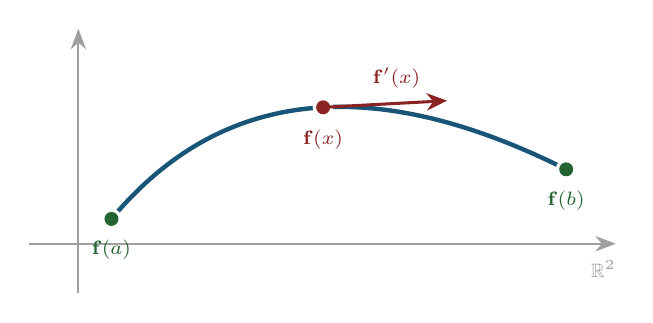
\begin{tikzpicture}[scale=1.05]
    % light axes
    \draw[axisln] (-0.6,0) -- (6.5,0);
    \draw[axisln] (0,-0.6) -- (0,2.6);
    \node[gray!75, font=\scriptsize, below] at (6.35,-0.08) {$\mathbb{R}^2$};
    % curve
    \draw[curveln, defcolor] (0.4,0.3) .. controls (1.9,2.1) and (3.9,1.9) .. (5.9,0.9);
    % endpoints
    \dotpt{proofcolor}{(0.4,0.3)}
    \node[proofcolor, below, font=\scriptsize] at (0.4,0.16) {$\mathbf{f}(a)$};
    \dotpt{proofcolor}{(5.9,0.9)}
    \node[proofcolor, below, font=\scriptsize] at (5.9,0.76) {$\mathbf{f}(b)$};
    % moving point + tangent
    \dotpt{thmcolor}{(2.96,1.65)}
    \node[thmcolor, below, font=\scriptsize] at (2.96,1.5) {$\mathbf{f}(x)$};
    \draw[guide, thmcolor] (2.96,1.65) -- (4.46,1.73);
    \node[thmcolor, above, font=\scriptsize] at (3.85,1.76) {$\mathbf{f}'(x)$};
  \end{tikzpicture}
  \end{center}

  \vspace{0.2em}
  \begin{center}
    \begin{hlbox}
    A curve $\mathbf{f}\colon [a,b] \to \mathbb{R}^2$; \ its derivative
    $\mathbf{f}'(x)$ is the \alert{velocity vector} of the motion.
    \end{hlbox}
  \end{center}

  \note{
    Here is the picture to keep in mind throughout the episode. The blue
    curve is the image of a function "f" defined on the interval from
    "a" to "b" with values in the plane: as "t" runs through the
    interval, the point "f" of "t" traces the curve. The two green dots
    mark the starting point, "f" of "a", and the ending point, "f" of
    "b". The red dot is the position "f" of "x" at some intermediate
    time "x", and the red arrow attached to it is the derivative "f"
    prime of "x". It points in the direction of motion, tangent to the
    curve, and its length is the instantaneous speed. So for curves, the
    derivative is not a slope; it is a velocity vector. With this
    picture in mind, let's define it properly.
  }
\end{frame}
}

{
\usebackgroundtemplate{%
  
\includegraphics[width=\paperwidth,height=\paperheight,keepaspectratio=false]{chapter_05_bg_02.png}%
}
\section{Vector-Valued Derivatives}

% --- Build 1/2 ---
\begin{frame}{Remarks 5.16: The Complex Case}
  \begin{remblock}{Remarks 5.16 (complex functions)}
    Definition 5.1 applies \alert{without any change} to complex
    functions $f$ on $[a,b]$, and Theorems 5.2 and 5.3, together with
    their proofs, remain valid.
  \end{remblock}

  \note{
    We begin with complex valued functions, following Remarks 5.16. The
    gray box records a pleasant fact: the definition of the derivative,
    Definition 5.1, makes sense word for word for a complex valued
    function on an interval, since we can subtract complex numbers,
    divide by the real number "t" minus "x", and take limits. Recall
    also Theorem 5.2, which says a function differentiable at a point is
    continuous there, and Theorem 5.3, the sum, product, and quotient
    rules. Both theorems, and even their proofs, remain valid for
    complex functions with no changes. Next, let's see how the complex
    case reduces to a pair of real cases.
  }
\end{frame}

% --- Build 2/2 ---
\begin{frame}{Remarks 5.16: The Complex Case}
  \begin{remblock}{Remarks 5.16 (complex functions)}
    Definition 5.1 applies \alert{without any change} to complex
    functions $f$ on $[a,b]$, and Theorems 5.2 and 5.3, together with
    their proofs, remain valid.
  \end{remblock}

  \begin{remblock}{Real and imaginary parts}
    If $f(t) = f_1(t) + i f_2(t)$ with $f_1, f_2$ real, then
    \begin{equation}
      f'(x) = f_1'(x) + i f_2'(x);
      \tag{29}
    \end{equation}
    $f$ is differentiable at $x$ \ $\Longleftrightarrow$ \
    both $f_1$ and $f_2$ are differentiable at $x$.
  \end{remblock}

  \note{
    Now write "f" of "t" as "f" sub 1 of "t" plus "i" times "f" sub 2 of
    "t", where "f" sub 1 is the real part and "f" sub 2 is the imaginary
    part. Equation 29 says that differentiation acts on the two parts
    separately: the derivative of "f" is the derivative of the real part
    plus "i" times the derivative of the imaginary part. Moreover, "f"
    is differentiable at "x" if and only if both parts are
    differentiable at "x". So a complex derivative is nothing more
    mysterious than two real derivatives computed side by side. The same
    idea handles vector values, as we see next.
  }
\end{frame}

\begin{frame}{The Vector Case: $\mathbf{f}$ Maps $[a,b]$ into $\mathbb{R}^k$}
  \begin{defblock}{The derivative of a vector-valued function}
    Apply Definition 5.1 verbatim: the difference quotient
    \[
      \boldsymbol{\phi}(t) = \frac{\mathbf{f}(t) - \mathbf{f}(x)}{t - x}
    \]
    is now, for each $t$, a \alert{point in $\mathbb{R}^k$}.
    Then $\mathbf{f}'(x)$ is that point of $\mathbb{R}^k$ (if there is
    one) for which
    \begin{equation}
      \lim_{t \to x}
      \left|\frac{\mathbf{f}(t) - \mathbf{f}(x)}{t - x}
      - \mathbf{f}'(x)\right| = 0.
      \tag{30}
    \end{equation}
  \end{defblock}

  \vspace{0.3em}
  \hl{$\mathbf{f}'$ is again a function with values in $\mathbb{R}^k$.}

  \note{
    Passing to vector valued functions in general, let "f" map the
    interval into "R" to the power "k". We may still apply Definition
    5.1. Recall that definition formed the quotient: "f" of "t" minus
    "f" of "x", divided by "t" minus "x". The numerator is now a vector,
    the difference of two points in "k" dimensional space, and dividing
    by the real number "t" minus "x" just rescales it; so the difference
    quotient is, for each "t", a point of "R" to the power "k".
    Equation 30 on the slide makes the limit precise: "f" prime of "x"
    is that point of the space, if one exists, for which the norm of the
    difference quotient minus "f" prime of "x" tends to zero as "t"
    approaches "x". The limit is taken with respect to the norm of the
    space. And as the last line notes, the derivative "f" prime is
    again a vector valued function. Just as in the complex case,
    everything can be read off the components.
  }
\end{frame}

\begin{frame}{Componentwise Differentiation}
  \begin{remblock}{Components (as in Theorem 4.10)}
    If $f_1, \dots, f_k$ are the components of $\mathbf{f}$, then
    \begin{equation}
      \mathbf{f}' = (f_1', \dots, f_k'),
      \tag{31}
    \end{equation}
    and $\mathbf{f}$ is differentiable at $x$ \
    $\Longleftrightarrow$ \ each of $f_1, \dots, f_k$ is
    differentiable at $x$.
  \end{remblock}

  \vspace{0.4em}
  \begin{hlbox}
  \textbf{Consequence:} for \emph{definitions and algebra}, vector
  calculus reduces to $k$ real problems.
  \end{hlbox}

  \note{
    Here is the cleanest way to think about vector derivatives. Recall
    from Theorem 4.10 that a vector valued function is the same thing as
    a list of "k" real functions, its components "f" sub 1 through "f"
    sub "k". Equation 31 says the derivative is computed componentwise:
    "f" prime is the vector whose components are the derivatives of the
    components. And "f" is differentiable at "x" if and only if every
    single component is differentiable at "x". So, as the bottom line
    says, as far as definitions and algebraic rules are concerned,
    vector calculus is just "k" copies of real calculus running in
    parallel. Let's record exactly which theorems carry over.
  }
\end{frame}

% --- Build 1/2 ---
\begin{frame}{What Survives}
  \begin{hlbox}
  \begin{itemize}
    \item Theorem 5.2: \ differentiable at $x$ $\Rightarrow$ continuous
      at $x$
    \item Theorem 5.3(a): \
      $(\mathbf{f} + \mathbf{g})'(x) = \mathbf{f}'(x) + \mathbf{g}'(x)$
  \end{itemize}
  \end{hlbox}

  \note{
    So what survives in the vector setting? First, Theorem 5.2:
    differentiability at a point still implies continuity at that point.
    This is clear componentwise, since each component is differentiable,
    hence continuous. Second, Theorem 5.3 part "a", the sum rule: the
    derivative of a sum of two vector valued functions is the sum of the
    derivatives. Again, nothing surprising happens in any component.
    The product rule needs one small adjustment, which we look at next.
  }
\end{frame}

% --- Build 2/2 ---
\begin{frame}{What Survives}
  \begin{hlbox}
  \begin{itemize}
    \item Theorem 5.2: \ differentiable at $x$ $\Rightarrow$ continuous
      at $x$
    \item Theorem 5.3(a): \
      $(\mathbf{f} + \mathbf{g})'(x) = \mathbf{f}'(x) + \mathbf{g}'(x)$
    \item Theorem 5.3(b), with $fg$ replaced by the \alert{inner
      product} (Def. 4.3):
      \[
        (\mathbf{f} \cdot \mathbf{g})'(x)
        = \mathbf{f}'(x) \cdot \mathbf{g}(x)
        + \mathbf{f}(x) \cdot \mathbf{g}'(x)
      \]
  \end{itemize}
  \end{hlbox}

  \note{
    The product rule, Theorem 5.3 part "b", also survives, provided we
    interpret the product correctly. Two vectors cannot be multiplied to
    give another vector, but they do have an inner product, the sum of
    the products of corresponding components, as in Definition 4.3. With
    the product "f" "g" replaced by the inner product, the familiar
    formula holds: the derivative of "f" dot "g" is "f" prime dot "g"
    plus "f" dot "g" prime. Note there is no analogue of part "c", the
    quotient rule, simply because we cannot divide by a vector. So far,
    the story has been remarkably smooth. That is about to change.
  }
\end{frame}

\begin{frame}{Where the Story Turns}
  \begin{hlbox}
  \begin{itemize}
    \item The \alert{mean value theorem} (5.10) \emph{fails} for
      complex-valued functions \ (Example 5.17)
    \item \alert{L'Hospital's rule} (5.13) \emph{fails} for
      complex-valued functions \ (Example 5.18)
  \end{itemize}

  \vspace{0.5em}
  Already for $k = 2$, equality-type theorems break
  down.
  \end{hlbox}

  \note{
    When we turn to the mean value theorem, however, and to one of its
    consequences, Lopital's rule, the situation changes completely. The
    two bullets on the slide announce the program for the next two
    sections of the episode. Example 5.17 will exhibit a complex valued
    function for which the mean value theorem, Theorem 5.10, fails
    outright. Example 5.18 will do the same for Lopital's rule, Theorem
    5.13. And note how little room is needed for these failures: the
    complex plane is just two dimensional space, so the smallest
    possible step beyond the real line is already enough to break both
    theorems. Let's see the first counterexample.
  }
\end{frame}
}

{
\usebackgroundtemplate{%
  
\includegraphics[width=\paperwidth,height=\paperheight,keepaspectratio=false]{chapter_05_bg_03.png}%
}
\section{The Mean Value Theorem Fails}

\begin{frame}{Example 5.17: A Trip Around the Circle}
  \begin{exblock}{Example 5.17}
    Define, for real $x$,
    \begin{equation}
      f(x) = e^{ix} = \cos x + i \sin x.
      \tag{32}
    \end{equation}
  \end{exblock}

  \vspace{0.4em}
  \begin{hlbox}
  \begin{itemize}
    \item Take (32) as the \emph{definition} of $e^{ix}$
      (full discussion in Chap.~8)
    \item As $x$ increases, $f(x)$ moves along the \alert{unit circle}
  \end{itemize}
  \end{hlbox}

  \note{
    Here is Rudin's first counterexample, Example 5.17. Equation 32
    defines, for real "x", the function "f" of "x" equals "e" to the
    power "i" "x", which by definition means cosine of "x" plus "i"
    times sine of "x". As the first bullet says, we simply take this
    formula as the definition of the complex exponential; the full
    theory of these functions comes in Chapter 8. The geometric picture
    is the second bullet: since cosine squared plus sine squared equals
    one, the value "f" of "x" always has absolute value one, so as "x"
    increases the point "f" of "x" travels around the unit circle in
    the complex plane. Now let's compute the two quantities that appear
    in the mean value theorem.
  }
\end{frame}

% --- Build 1/3 ---
\begin{frame}{Example 5.17: Zero Displacement, Unit Speed}
  \begin{exblock}{The displacement over $[0, 2\pi]$}
    \begin{equation}
      f(2\pi) - f(0) = 1 - 1 = 0
      \tag{33}
    \end{equation}
  \end{exblock}

  \note{
    First, the displacement. At time zero, "e" to the power zero is one.
    At time two pi, cosine of two pi is one and sine of two pi is zero,
    so the value is again one. Equation 33 records the result: "f" of
    two pi minus "f" of zero equals one minus one, which is zero. After
    one full lap around the circle, the function returns exactly to its
    starting point; the total displacement vanishes. Next, the
    derivative.
  }
\end{frame}

% --- Build 2/3 ---
\begin{frame}{Example 5.17: Zero Displacement, Unit Speed}
  \begin{exblock}{The displacement over $[0, 2\pi]$}
    \begin{equation}
      f(2\pi) - f(0) = 1 - 1 = 0
      \tag{33}
    \end{equation}
  \end{exblock}

  \begin{exblock}{The derivative}
    \begin{equation}
      f'(x) = i e^{ix},
      \qquad \text{so that} \quad
      \alert{|f'(x)| = 1} \ \text{ for all real } x.
      \tag{34}
    \end{equation}
  \end{exblock}

  \note{
    Differentiate the real and imaginary parts: the derivative of cosine
    is minus sine, and the derivative of sine is cosine, so "f" prime of
    "x" is minus sine of "x" plus "i" times cosine of "x". Factoring out
    "i" gives equation 34: "f" prime of "x" equals "i" times "e" to the
    power "i" "x". Both factors have absolute value one, so the absolute
    value of the derivative is exactly one at every real "x". In the
    language of motion: the point travels at unit speed at every
    instant, and in particular the derivative is never zero.
  }
\end{frame}

% --- Build 3/3 ---
\begin{frame}{Example 5.17: Zero Displacement, Unit Speed}
  \begin{exblock}{The displacement over $[0, 2\pi]$}
    \begin{equation}
      f(2\pi) - f(0) = 1 - 1 = 0
      \tag{33}
    \end{equation}
  \end{exblock}

  \begin{exblock}{The derivative}
    \begin{equation}
      f'(x) = i e^{ix},
      \qquad \text{so that} \quad
      \alert{|f'(x)| = 1} \ \text{ for all real } x.
      \tag{34}
    \end{equation}
  \end{exblock}

  \vspace{0.3em}
  \begin{hlbox}
  Theorem 5.10 would require $f(2\pi) - f(0) = 2\pi f'(x)$, i.e.\
  $f'(x) = 0$ for some $x$ --- \alert{impossible}.
  Thus \alert{Theorem 5.10 fails} for complex functions.
  \end{hlbox}

  \note{
    Now put the two computations side by side. If the mean value
    theorem, Theorem 5.10, were true for complex functions, there would
    be a point "x" between zero and two pi with "f" of two pi minus "f"
    of zero equal to two pi times "f" prime of "x". The left side is
    zero by equation 33, so "f" prime of "x" would have to vanish
    somewhere. But equation 34 says the derivative has absolute value
    one everywhere; it never vanishes. The conclusion stands at the
    bottom of the slide: Theorem 5.10 fails to hold for complex valued
    functions. The next slide shows how obvious this failure is once
    you draw the picture.
  }
\end{frame}

\begin{frame}[c]{The Picture: Motion on the Unit Circle}
  \begin{center}
  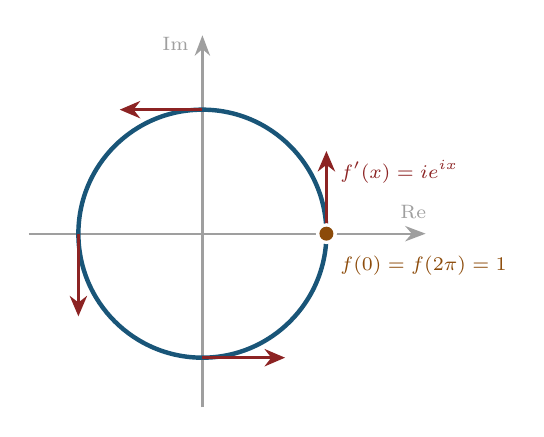
\begin{tikzpicture}[scale=1.05]
    % axes
    \draw[axisln] (-2.1,0) -- (2.7,0);
    \draw[axisln] (0,-2.1) -- (0,2.4);
    \node[gray!75, font=\scriptsize, above] at (2.55,0.06) {Re};
    \node[gray!75, font=\scriptsize, left] at (-0.05,2.3) {Im};
    % circle
    \draw[curveln, defcolor] (0,0) circle (1.5);
    % tangent arrows
    \draw[guide, thmcolor] (0,1.5) -- (-1.0,1.5);
    \draw[guide, thmcolor] (-1.5,0) -- (-1.5,-1.0);
    \draw[guide, thmcolor] (0,-1.5) -- (1.0,-1.5);
    \draw[guide, thmcolor] (1.5,0) -- (1.5,1.0);
    \node[thmcolor, right, font=\scriptsize] at (1.55,0.75) {$f'(x) = ie^{ix}$};
    % start/end point
    \dotpt{excolor}{(1.5,0)}
    \node[excolor, font=\scriptsize, anchor=north west] at (1.55,-0.15)
      {$f(0) = f(2\pi) = 1$};
  \end{tikzpicture}
  \end{center}

  \vspace{0.1em}
  \begin{center}
    \begin{hlbox}
    Displacement over $[0,2\pi]$: \alert{zero}. \quad
    Speed at every instant: \alert{one}.
    \end{hlbox}
  \end{center}

  \note{
    Here is the whole example in one picture. The blue circle is the
    unit circle in the complex plane, with the real axis pointing right
    and the imaginary axis pointing up. The orange dot on the right is
    the number one: it is both the starting point, "f" of zero, and the
    ending point, "f" of two pi. The red arrows are the velocity vectors
    at four moments of the trip; each is tangent to the circle, has
    length one, and points counterclockwise. Think of a car driving one
    full lap around a circular track at constant speed. Its average
    velocity over the lap is zero, because it ends where it began, but
    at no instant is its actual velocity zero. For real functions the
    mean value theorem forbids this; in the plane, nothing forbids it,
    because the velocity can point in different directions at different
    times and still never vanish. Let's now break Lopital's rule.
  }
\end{frame}
}

{
\usebackgroundtemplate{%
  
\includegraphics[width=\paperwidth,height=\paperheight,keepaspectratio=false]{chapter_05_bg_04.png}%
}
\section{L'Hospital's Rule Fails}

\begin{frame}{Example 5.18: The Setup}
  \begin{exblock}{Example 5.18}
    On the segment $(0,1)$, define $f(x) = x$ and
    \begin{equation}
      g(x) = x + x^2 e^{i/x^2}.
      \tag{35}
    \end{equation}
  \end{exblock}

  \vspace{0.3em}
  \begin{hlbox}
  Since $|e^{it}| = 1$ for all real $t$: \quad
  $\dfrac{f(x)}{g(x)} = \dfrac{1}{1 + x\,e^{i/x^2}}$
  \ and \ $\bigl|x\,e^{i/x^2}\bigr| = x \to 0$, so
  \begin{equation}
    \lim_{x \to 0} \frac{f(x)}{g(x)} = 1.
    \tag{36}
  \end{equation}
  \end{hlbox}

  \note{
    Now for the second counterexample, Example 5.18, aimed at Lopital's
    rule. On the open segment from zero to one, define two functions.
    The first is as simple as possible: "f" of "x" equals "x". The
    second, in equation 35, is "g" of "x" equals "x" plus "x" squared
    times "e" to the power "i" over "x" squared. That exponential
    factor has absolute value one for every real exponent; it just
    spins around the unit circle. So "g" is the identity function plus
    a perturbation of size "x" squared, which is tiny near zero. The
    line below the block divides through by "x": the ratio of "f" to
    "g" is one over the quantity one plus "x" times the exponential
    factor, and that correction has absolute value "x", which tends to
    zero. Equation 36 follows: the ratio of the two functions tends to
    one. Now watch what the derivatives do.
  }
\end{frame}

\begin{frame}{Example 5.18: The Derivative of $g$ Blows Up}
  \begin{exblock}{Differentiate (35)}
    \begin{equation}
      g'(x) = 1 + \left\{2x - \frac{2i}{x}\right\} e^{i/x^2}
      \qquad (0 < x < 1),
      \tag{37}
    \end{equation}
    so that
    \begin{equation}
      |g'(x)| \geq \left|2x - \frac{2i}{x}\right| - 1 \geq \frac{2}{x} - 1.
      \tag{38}
    \end{equation}
  \end{exblock}

  \vspace{0.3em}
  \hl{In particular $g'(x) \neq 0$ on $(0,1)$, and $|g'(x)| \to \infty$ as $x \to 0$.}

  \note{
    Differentiating equation 35 gives equation 37. The derivative of
    the first term "x" is one. For the second term, the product rule
    produces two "x" times the exponential factor, and the chain rule
    applied to the exponent "i" over "x" squared produces the term
    minus two "i" over "x" times the same factor. Now estimate the
    size, in equation 38. The curly bracket has absolute value the
    square root of four "x" squared plus four over "x" squared, which
    is at least two over "x"; the exponential factor has absolute value
    one; and by the triangle inequality, subtracting the term one can
    cost at most one. So the absolute value of "g" prime of "x" is at
    least two over "x" minus one. Two things follow, as the last line
    says. First, "g" prime never vanishes on our segment, so the
    hypothesis of Lopital's rule is satisfied. Second, the derivative
    actually blows up near zero. That is the key to the failure.
  }
\end{frame}

\begin{frame}{Example 5.18: The Punch Line}
  \begin{exblock}{The ratio of derivatives}
    Since $f'(x) = 1$, (38) gives
    \begin{equation}
      \left|\frac{f'(x)}{g'(x)}\right| = \frac{1}{|g'(x)|}
      \leq \frac{x}{2 - x},
      \tag{39}
    \end{equation}
    and so
    \begin{equation}
      \lim_{x \to 0} \frac{f'(x)}{g'(x)} = 0.
      \tag{40}
    \end{equation}
  \end{exblock}

  \vspace{0.3em}
  \hl{By (36) and (40): \ $\dfrac{f}{g} \to \alert{1}$ \ but \
  $\dfrac{f'}{g'} \to \alert{0}$. \quad \alert{L'Hospital's rule fails.}}

  \note{
    The punch line is now a one-liner. The derivative of "f" is
    constantly one, so the absolute value of the ratio "f" prime over
    "g" prime is just the reciprocal of the absolute value of "g"
    prime. By equation 38 that reciprocal is at most "x" divided by two
    minus "x", which is equation 39, and this bound tends to zero.
    Equation 40 records the conclusion: the ratio of the derivatives
    tends to zero. Now compare. Equation 36 said the ratio of the
    functions tends to one. Equation 40 says the ratio of the
    derivatives tends to zero. Lopital's rule, which claims the two
    limits agree, fails in this case, even though all its hypotheses
    that make sense here are satisfied. What exactly went wrong? Let's
    take a moment to understand the mechanism.
  }
\end{frame}

\begin{frame}{What Went Wrong?}
  \begin{remblock}{The mechanism behind both failures}
    \begin{itemize}
      \item The perturbation $x^2 e^{i/x^2}$ is \alert{small}:
        $\ |x^2 e^{i/x^2}| = x^2 \to 0$
      \item Its derivative is \alert{huge}: size $\approx 2/x \to \infty$:
        ever-faster \emph{spinning}
      \item A vector-valued function can move at high speed while
        \emph{staying close to a point}
    \end{itemize}
  \end{remblock}

  \note{
    Here is the mechanism, and it is the same one in both examples. The
    perturbation that we added to "x" is "x" squared times the spinning
    exponential factor. The first bullet says it is small: its absolute
    value is "x" squared, which vanishes rapidly as "x" tends to zero.
    The second bullet says its derivative is nevertheless enormous, of
    size roughly two over "x", because the exponent "i" over "x"
    squared changes faster and faster: the value spins around a tiny
    circle at a furious rate. And that is the essential difference from
    the real line, summarized in the third bullet: a vector valued
    function can have a large derivative while staying near one point,
    by rapidly changing direction. A real function that moves fast must
    actually go somewhere. This insight also tells us what we can hope
    to save: not an equality involving the derivative at one point, but
    an inequality bounding the displacement by the speed. That is
    exactly Theorem 5.19.
  }
\end{frame}
}

{
\usebackgroundtemplate{%
  
\includegraphics[width=\paperwidth,height=\paperheight,keepaspectratio=false]{chapter_05_bg_05.png}%
}
\section{The Inequality That Survives}

\begin{frame}{Salvaging the Mean Value Theorem}
  \begin{remblock}{A consequence of Theorem 5.10 (real case)}
    \begin{equation}
      |f(b) - f(a)| \leq (b - a) \sup_{a < x < b} |f'(x)|
      \tag{41}
    \end{equation}
  \end{remblock}

  \vspace{0.4em}
  \begin{hlbox}
  \begin{itemize}
    \item For applications, (41) is \emph{almost as useful} as
      Theorem 5.10 itself
    \item And --- unlike (5.10) --- it \alert{remains true} for
      vector-valued functions
  \end{itemize}
  \end{hlbox}

  \note{
    However, there is a consequence of the mean value theorem which
    survives, and it is the one that gets used in practice all the
    time. For a real function, Theorem 5.10 immediately implies the
    inequality in equation 41: the total displacement, "f" of "b" minus
    "f" of "a" in absolute value, is at most the length of the interval
    times the supremum of the absolute value of the derivative. In
    words: the net displacement is at most time elapsed times top speed.
    The first bullet makes a practical point: in applications one
    rarely needs the exact mean value equality; this estimate is almost
    always enough. And the second bullet is the good news of this
    section: unlike the mean value theorem itself, this inequality
    remains true for vector valued functions. That is the content of
    Theorem 5.19, our final theorem of the chapter.
  }
\end{frame}

\begin{frame}{Theorem 5.19: The Mean Value Inequality}
  \begin{thmblock}{Theorem 5.19}
    Suppose $\mathbf{f}$ is a continuous mapping of $[a,b]$ into
    $\mathbb{R}^k$ and $\mathbf{f}$ is differentiable in $(a,b)$. Then
    there exists $x \in (a,b)$ such that
    \[
      |\mathbf{f}(b) - \mathbf{f}(a)| \leq (b - a)\,|\mathbf{f}'(x)|.
    \]
  \end{thmblock}

  \vspace{0.4em}
  \begin{hlbox}
  \textbf{Check against Example 5.17:} \
  $|f(2\pi) - f(0)| = 0 \leq 2\pi \cdot 1$
  \ (inequality, not equality!)
  \end{hlbox}

  \note{
    Here is the statement. Suppose "f" is a continuous mapping of the
    closed interval from "a" to "b" into "R" to the power "k", and "f"
    is differentiable at every interior point. Then there exists a
    point "x" strictly between "a" and "b" such that the norm of "f" of
    "b" minus "f" of "a" is at most "b" minus "a" times the norm of "f"
    prime of "x". Notice the shape: it is exactly the mean value
    theorem with the equality relaxed to an inequality between norms.
    Even better, it still produces a single point "x"; we do not even
    need a supremum on the right hand side. The line at the bottom
    checks the theorem against our circle example: there the left side
    is zero and the right side is two pi, and zero is certainly at most
    two pi. The inequality is comfortably true, while the equality
    version failed. Let's see how to prove it.
  }
\end{frame}

\begin{frame}{Proof Strategy}
  \begin{hlbox}
  \textbf{Goal:} find $x \in (a,b)$ with
  $|\mathbf{f}(b) - \mathbf{f}(a)| \leq (b-a)\,|\mathbf{f}'(x)|$.

  \vspace{0.5em}
  \textbf{Approach:}
  \begin{enumerate}
    \item Let $\mathbf{z} = \mathbf{f}(b) - \mathbf{f}(a)$ be the
      \alert{displacement vector}
    \item Project the motion onto $\mathbf{z}$: \
      $\varphi(t) = \mathbf{z} \cdot \mathbf{f}(t)$ is \alert{real-valued}
    \item Apply the \alert{real} mean value theorem to $\varphi$
    \item Finish with the \alert{Schwarz inequality}
  \end{enumerate}

  \vspace{0.4em}
  \textbf{Technique:} reduction to the real case by projection.
  \end{hlbox}

  \note{
    Before the formal proof, here is the plan of attack. The trouble
    with the mean value theorem in higher dimensions is that we cannot
    apply it to a vector valued function directly. The trick is to
    convert the vector problem into a real one, and to do it without
    throwing away the information we care about. Step one: form the
    displacement vector "z", the difference between the endpoint values
    of "f". Step two: project the whole motion onto that direction, by
    taking the inner product of "z" with "f" of "t"; this produces a
    real valued function phi of "t" that measures progress in the
    direction of the total displacement. Step three: apply the ordinary
    mean value theorem, which is available for the real function phi.
    Step four: convert the resulting statement back into a statement
    about norms using the Schwarz inequality from Chapter 1. This
    technique, reducing a vector problem to a real one by projecting,
    is worth remembering; it reappears in Chapter 6. Here is the
    projection in a picture.
  }
\end{frame}

\begin{frame}[c]{The Projection Idea}
  \begin{center}
  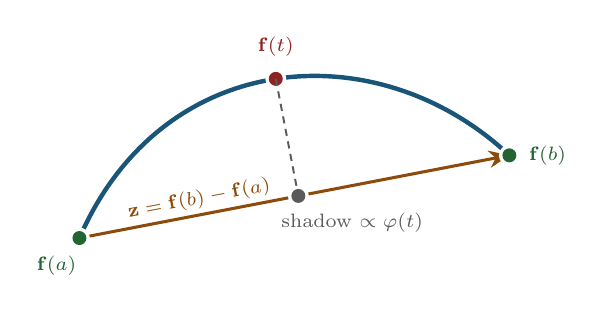
\begin{tikzpicture}[scale=1.05]
    % curve
    \draw[curveln, defcolor] (0,0) .. controls (1.0,2.3) and (3.6,2.5) .. (5.2,1.0);
    % chord (displacement)
    \draw[guide, excolor] (0,0) -- (5.2,1.0);
    \node[excolor, font=\scriptsize, rotate=10.9] at (1.45,0.47)
      {$\mathbf{z} = \mathbf{f}(b) - \mathbf{f}(a)$};
    % endpoints
    \dotpt{proofcolor}{(0,0)}
    \node[proofcolor, below left, font=\scriptsize] at (0.08,-0.1) {$\mathbf{f}(a)$};
    \dotpt{proofcolor}{(5.2,1.0)}
    \node[proofcolor, right, font=\scriptsize] at (5.32,1.0) {$\mathbf{f}(b)$};
    % moving point + projection
    \dotpt{thmcolor}{(2.375,1.925)}
    \node[thmcolor, above, font=\scriptsize] at (2.375,2.08) {$\mathbf{f}(t)$};
    \draw[projln, remcolor] (2.375,1.925) -- (2.648,0.509);
    \dotpt{remcolor}{(2.648,0.509)}
    \node[remcolor, font=\scriptsize, anchor=north] at (3.3,0.42)
      {shadow $\propto \varphi(t)$};
  \end{tikzpicture}
  \end{center}

  \vspace{0.1em}
  \begin{center}
    \begin{hlbox}
    $\varphi(t) = \mathbf{z} \cdot \mathbf{f}(t)$: \ a \alert{real}
    function tracking progress along the chord.
    \end{hlbox}
  \end{center}

  \note{
    Let's look at the picture. The blue curve is the path traced by "f"
    between the two green endpoints, "f" of "a" and "f" of "b". The
    orange arrow is the chord joining them: the displacement vector
    "z", equal to "f" of "b" minus "f" of "a". The red dot is the
    moving point "f" of "t" at some intermediate time, and the gray
    dashed line drops from it perpendicularly onto the chord; the gray
    dot at its foot is the shadow of the moving point on the chord
    direction. The real function phi of "t", defined as "z" dot "f" of
    "t", is proportional to how far along the chord that shadow has
    advanced. The curve may wander wherever it likes, but its shadow
    moves along a fixed line, and a motion along a line is a real
    valued function, exactly what the mean value theorem can handle.
    Now we carry out the plan.
  }
\end{frame}

\begin{frame}{Proof of Theorem 5.19 --- Step 1: Project onto the Chord}
  \begin{proofblock}{Step 1: A real-valued auxiliary function}
    Put $\mathbf{z} = \mathbf{f}(b) - \mathbf{f}(a)$, and define
    \[
      \varphi(t) = \mathbf{z} \cdot \mathbf{f}(t) \qquad (a \leq t \leq b).
    \]
    Then $\varphi$ is \alert{real-valued}, continuous on $[a,b]$,
    differentiable in $(a,b)$, with
    $\ \varphi'(t) = \mathbf{z} \cdot \mathbf{f}'(t)$.
  \end{proofblock}

  \note{
    Step one. Put "z" equal to "f" of "b" minus "f" of "a", the fixed
    displacement vector, and define phi of "t" as the inner product of
    "z" with "f" of "t", for "t" in the closed interval. The inner
    product of a fixed vector with a continuous vector valued function
    is a real valued continuous function, and by the product rule for
    inner products, which we saw survives in the vector setting, phi is
    differentiable at interior points with derivative "z" dot "f" prime
    of "t"; the term involving the derivative of the constant vector
    "z" simply drops out. So phi inherits from "f" exactly the
    hypotheses that the real mean value theorem needs. Let's apply it.
  }
\end{frame}

\begin{frame}{Proof of Theorem 5.19 --- Step 2: Apply the Real MVT}
  \begin{proofblock}{Step 2: The mean value theorem for $\varphi$}
    By Theorem 5.10, there is a point $x \in (a,b)$ with
    \[
      \varphi(b) - \varphi(a) = (b - a)\,\varphi'(x)
      = (b - a)\,\mathbf{z} \cdot \mathbf{f}'(x).
    \]
  \end{proofblock}

  \note{
    Step two. The function phi is a real valued continuous function on
    the closed interval, differentiable inside, so the mean value
    theorem, Theorem 5.10, applies to it; this is precisely the point of
    having projected. It produces a point "x" strictly between "a" and
    "b" at which phi of "b" minus phi of "a" equals "b" minus "a" times
    the derivative of phi at "x", and by step one that derivative is
    "z" dot "f" prime of "x". So the increment of phi is now expressed
    through the derivative of "f" at a single interior point. Next we
    compute that same increment directly.
  }
\end{frame}

\begin{frame}{Proof of Theorem 5.19 --- Step 3: Compute the Increment}
  \begin{proofblock}{Step 3: The increment of $\varphi$ is $|\mathbf{z}|^2$}
    On the other hand,
    \[
      \varphi(b) - \varphi(a)
      = \mathbf{z} \cdot \mathbf{f}(b) - \mathbf{z} \cdot \mathbf{f}(a)
      = \mathbf{z} \cdot \bigl(\mathbf{f}(b) - \mathbf{f}(a)\bigr)
      = \mathbf{z} \cdot \mathbf{z}
      = |\mathbf{z}|^2.
    \]
  \end{proofblock}

  \note{
    Step three is a direct computation of the same quantity. By
    definition, phi of "b" minus phi of "a" is "z" dot "f" of "b" minus
    "z" dot "f" of "a". The inner product is linear, so we can factor
    out "z": this is "z" dot the difference "f" of "b" minus "f" of
    "a". But that difference is exactly "z" itself; that is how we
    chose "z". So the increment equals "z" dot "z", which is the square
    of the norm of "z". Notice the effect of choosing the chord
    direction for the projection: the increment of phi captures the
    full length of the displacement, squared, with nothing lost.
    Combining steps two and three, the square of the norm of "z"
    equals "b" minus "a" times "z" dot "f" prime of "x". One
    inequality now finishes the proof.
  }
\end{frame}

\begin{frame}{Proof of Theorem 5.19 --- Step 4: Schwarz Inequality}
  \begin{proofblock}{Step 4: Conclusion}
    The Schwarz inequality now gives
    \[
      |\mathbf{z}|^2 = (b - a)\,|\mathbf{z} \cdot \mathbf{f}'(x)|
      \leq (b - a)\,|\mathbf{z}|\,|\mathbf{f}'(x)|.
    \]
    If $\mathbf{z} \neq \mathbf{0}$, divide by $|\mathbf{z}|$
    (if $\mathbf{z} = \mathbf{0}$, the conclusion is trivial):
    \[
      \boxed{\,|\mathbf{f}(b) - \mathbf{f}(a)| \leq
      (b - a)\,|\mathbf{f}'(x)|\,}
    \]
  \end{proofblock}

  \vspace{0.3em}
  \hl{This proves Theorem 5.19. \quad $\blacksquare$}

  \note{
    Step four. From the previous two steps, the square of the norm of
    "z" equals "b" minus "a" times "z" dot "f" prime of "x"; since the
    left side is nonnegative we may put absolute values around the
    right side. The Schwarz inequality, from Chapter 1, bounds the
    absolute value of an inner product by the product of the norms: "z"
    dot "f" prime of "x" is at most the norm of "z" times the norm of
    "f" prime of "x". If "z" is not the zero vector, divide both sides
    by its norm, and the boxed inequality appears: the norm of "f" of
    "b" minus "f" of "a" is at most "b" minus "a" times the norm of "f"
    prime of "x". If "z" happens to be the zero vector, the left side
    of the conclusion is zero and there is nothing to prove. The proof
    is complete: one projection, one mean value theorem, one Schwarz
    inequality. Let's summarize the episode.
  }
\end{frame}
}

{
\usebackgroundtemplate{%
  
\includegraphics[width=\paperwidth,height=\paperheight,keepaspectratio=false]{chapter_05_bg_06.png}%
}
\section{Summary}

% --- Build 1/3 ---
\begin{frame}{Summary}
  \begin{hlbox}
  \textbf{Key takeaways from this section:}
  \begin{itemize}
    \item \textbf{The derivative extends verbatim} to complex and
      $\mathbb{R}^k$-valued functions, and works \alert{componentwise}:
      $\mathbf{f}' = (f_1', \dots, f_k')$; Theorems 5.2 and 5.3(a),(b)
      (inner product) survive
  \end{itemize}
  \end{hlbox}

  \note{
    Let's review what we learned. First, the definition of the
    derivative passes to complex valued and vector valued functions
    without any change, and in practice everything is computed
    componentwise: the derivative of "f" is the vector of the
    derivatives of its components, and "f" is differentiable exactly
    when all components are. The basic theorems survive too:
    differentiability still implies continuity, the sum rule holds, and
    the product rule holds with the product interpreted as the inner
    product.
  }
\end{frame}

% --- Build 2/3 ---
\begin{frame}{Summary}
  \begin{hlbox}
  \textbf{Key takeaways from this section:}
  \begin{itemize}
    \item \textbf{The derivative extends verbatim} to complex and
      $\mathbb{R}^k$-valued functions, and works \alert{componentwise}:
      $\mathbf{f}' = (f_1', \dots, f_k')$; Theorems 5.2 and 5.3(a),(b)
      (inner product) survive
    \item \textbf{Two famous results fail:} the MVT
      ($f(x) = e^{ix}$: zero displacement, unit speed) and
      L'Hospital's rule ($g(x) = x + x^2e^{i/x^2}$:
      $f/g \to 1$ but $f'/g' \to 0$)
  \end{itemize}
  \end{hlbox}

  \note{
    Second, the failures. The mean value theorem breaks down already
    for complex valued functions: the exponential "e" to the power "i"
    "x" makes a full lap around the unit circle with zero total
    displacement while moving at unit speed throughout, so no point can
    witness the mean value equality. And Lopital's rule fails as well:
    with "g" equal to "x" plus a small but furiously spinning
    perturbation, the ratio of the functions tends to one while the
    ratio of the derivatives tends to zero. The moral: in the plane and
    beyond, a function can move fast while staying close to one point.
  }
\end{frame}

% --- Build 3/3 ---
\begin{frame}{Summary}
  \begin{hlbox}
  \textbf{Key takeaways from this section:}
  \begin{itemize}
    \item \textbf{The derivative extends verbatim} to complex and
      $\mathbb{R}^k$-valued functions, and works \alert{componentwise}:
      $\mathbf{f}' = (f_1', \dots, f_k')$; Theorems 5.2 and 5.3(a),(b)
      (inner product) survive
    \item \textbf{Two famous results fail:} the MVT
      ($f(x) = e^{ix}$: zero displacement, unit speed) and
      L'Hospital's rule ($g(x) = x + x^2e^{i/x^2}$:
      $f/g \to 1$ but $f'/g' \to 0$)
    \item \textbf{Theorem 5.19 saves the day:}
      $|\mathbf{f}(b) - \mathbf{f}(a)| \leq (b-a)\,|\mathbf{f}'(x)|$ ---
      proved by \alert{projection} onto the chord $+$ MVT $+$ Schwarz
  \end{itemize}

  \vspace{0.3em}
  \textbf{Coming up next:} Chapter 6 --- the Riemann--Stieltjes integral
  $\int_a^b f\,d\alpha$.
  \end{hlbox}

  \note{
    Third, the rescue. Theorem 5.19 keeps the practically useful half
    of the mean value theorem: the displacement of a vector valued
    function is bounded by the length of the interval times the norm of
    the derivative at some interior point. The proof pattern is worth
    remembering: project the motion onto the chord to get a real valued
    function, apply the ordinary mean value theorem to it, and finish
    with the Schwarz inequality. This completes Chapter 5. In the next
    episode we open Chapter 6 and take on integration: the
    Riemann-Stieltjes integral, which generalizes the familiar Riemann
    integral by integrating one function against another. The
    differentiation theory we just built will meet it head-on in the
    fundamental theorem of calculus. See you there.
  }
\end{frame}
}

\end{document}
